\documentclass[tikz,border=7pt]{standalone}
\usepackage{amsmath,amssymb}
\usetikzlibrary{calc}

\begin{document}
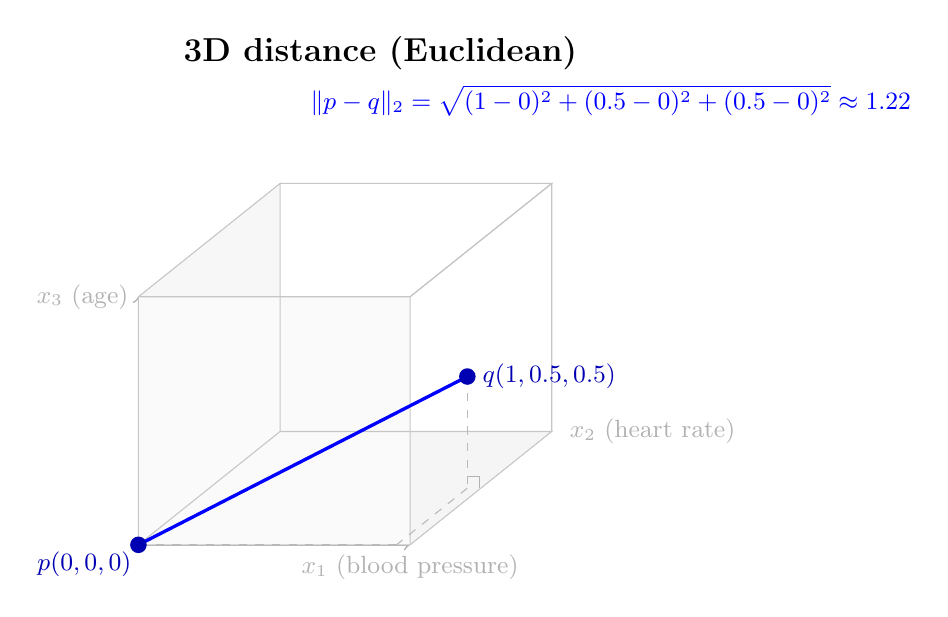
\begin{tikzpicture}[scale=3.0, every node/.style={font=\small}]
  %--- isometrische 3D-Projektion (nur 2D-TikZ)
  %   Basisrichtungen (x1, x2, x3) in die Bildebene
  \coordinate (O) at (0,0);
  \coordinate (E1) at (1.15,0.00);   % x1
  \coordinate (E2) at (0.60,0.48);   % x2
  \coordinate (E3) at (0.00,1.05);   % x3

  %--- Achsen
  \draw[->,gray!60, line width=0.6pt] (O) -- (E1) node[below] {$x_1$ (blood pressure)};
\draw[->,gray!60, line width=3.5pt] (O) -- (E2)
    node[anchor=west, xshift=3.5cm] {$x_2$ (heart rate)};


  \draw[->,gray!60, line width=0.6pt] (O) -- (E3) node[left]  {$x_3$ (age)};

  %--- Würfelkanten [0,1]^3
  \coordinate (A000) at (O);
  \coordinate (A100) at ($(O)+(E1)$);
  \coordinate (A010) at ($(O)+(E2)$);
  \coordinate (A001) at ($(O)+(E3)$);
  \coordinate (A110) at ($(O)+(E1)+(E2)$);
  \coordinate (A101) at ($(O)+(E1)+(E3)$);
  \coordinate (A011) at ($(O)+(E2)+(E3)$);
  \coordinate (A111) at ($(O)+(E1)+(E2)+(E3)$);

  % halbtransparente Rückwand/Seiten
  \fill[gray!8] (A000)--(A100)--(A110)--(A010)--cycle;         % Boden
  \fill[gray!6] (A000)--(A001)--(A011)--(A010)--cycle;         % linke Wand
  \fill[gray!4] (A000)--(A001)--(A101)--(A100)--cycle;         % rechte Wand

  % sichtbare Kanten
  \draw[gray!45, line width=0.4pt] (A000)--(A100)--(A110)--(A010)--cycle;
  \draw[gray!45, line width=0.4pt] (A000)--(A001)--(A011)--(A010);
  \draw[gray!45, line width=0.4pt] (A001)--(A101)--(A111)--(A011);
  \draw[gray!45, line width=0.4pt] (A100)--(A101)--(A111)--(A110);

  %--- Punkte p und q
  \coordinate (p) at (A000);                                % (0,0,0)
  \coordinate (q) at ($(O)+0.95*(E1)+0.50*(E2)+0.45*(E3)$); % ~ (1,0.5,0.5)

  % Projektionen von q
  \coordinate (q_xy) at ($(O)+0.95*(E1)+0.50*(E2)$);
  \coordinate (q_x)  at ($(O)+0.95*(E1)$);

  % Hilfslinien (gestrichelt)
  \draw[dashed,gray!55] (q) -- (q_xy);
  \draw[dashed,gray!55] (q_xy) -- (q_x);
  \draw[dashed,gray!55] (q_x) -- (p);

  % Rechtwinkelsymbol in der xy-Projektion
  \draw[gray!60, line width=0.35pt] ($(q_xy)+(0.05,0)$) -- ($(q_xy)+(0.05,0.05)$) -- ($(q_xy)+(0,0.05)$);

  % Distanz (3D-Diagonale)
  \draw[very thick, blue] (p) -- (q);

  % Punkte markieren + Labels
  \fill[blue!70!black] (p) circle (0.035) node[below left=-1pt] {$p(0,0,0)$};
  \fill[blue!70!black] (q) circle (0.035) node[right=2pt]       {$q(1,0.5,0.5)$};

  % Formel kompakt rechts oben
  \node[blue] at ($(A111)+(0.25,0.35)$)
    {$\displaystyle \|p-q\|_2=\sqrt{(1-0)^2+(0.5-0)^2+(0.5-0)^2}\approx1.22$};

  % Überschrift klein und links oben
  \node[anchor=west,font=\bfseries\large] at ($(A111)+(-1.6,0.55)$) {3D distance (Euclidean)};
\end{tikzpicture}
\end{document}
